\section{The \ours dataset} \label{sec:dataset}
%%%%%%%%%%%%%%%%%%%%

\label{sec:dataset_overview}

The \ours dataset consists of \numclaims scientific claims verified against a corpus of \numpapers abstracts.  Abstracts that support or refute each claim are annotated with rationales.  We describe our corpus creation and annotation process. Additional details on the corpus and data collection process can be found in Appendix \ref{sec:data_collection}, along with additional statistics on the dataset.

%%%%%%%%%%%%%%%%%%%%

\subsection{Data source and corpus construction}
\label{sec:data_source}

To construct \ours, we use S2ORC \cite{Lo2019GORCAL}, a publicly-available corpus of millions of scientific articles. To ensure that documents in our dataset are of high quality, we randomly sample articles from a manually curated collection of well-regarded journals spanning domains from basic science (e.g., \emph{Cell}, \emph{Nature}) to clinical medicine (e.g., \emph{JAMA}, \emph{BMJ}). We restrict to articles with at least 10 citations and with full text freely available. The resulting collection is referred to as our \textit{seed} set. We use the S2ORC citation graph to sample \emph{source citances} from \emph{citing articles} which cite these seed articles. If a citance cites other articles not in the seed set, we refer to these as \emph{co-cited} articles and add them to the corpus, as depicted in Figure \ref{fig:corpus}. The majority of citances used for \ours cite only the seed article (no co-cited articles), as we found in initial annotation experiments that these citances tended to yield specific, easy-to-verify claims.


%We focus on verifying claims against abstracts rather of full articles because (1) abstracts can be read much more quickly, and (2) it decreases ambiguity and mental burden for annotators, since a finding might be re-stated or alluded to multiple times throughout a paper.

% Ideally, we would use all of S2ORC as our corpus of abstracts. However, this would introduce many \emph{false negative retrievals}: abstracts containing evidence relevant to a given claim, but not mentioned in the claim's source citance. 

To expand the corpus, we identify five papers cited in the same paper as each source citance but in a different paragraph, and add these to the corpus as \emph{distractor abstracts}. These abstracts often discuss similar topics to the evidence documents, increasing the difficulty of abstract retrieval and making our metrics more accurately reflect the system's performance on a large research corpus.

\begin{figure}[t]
  \centering

  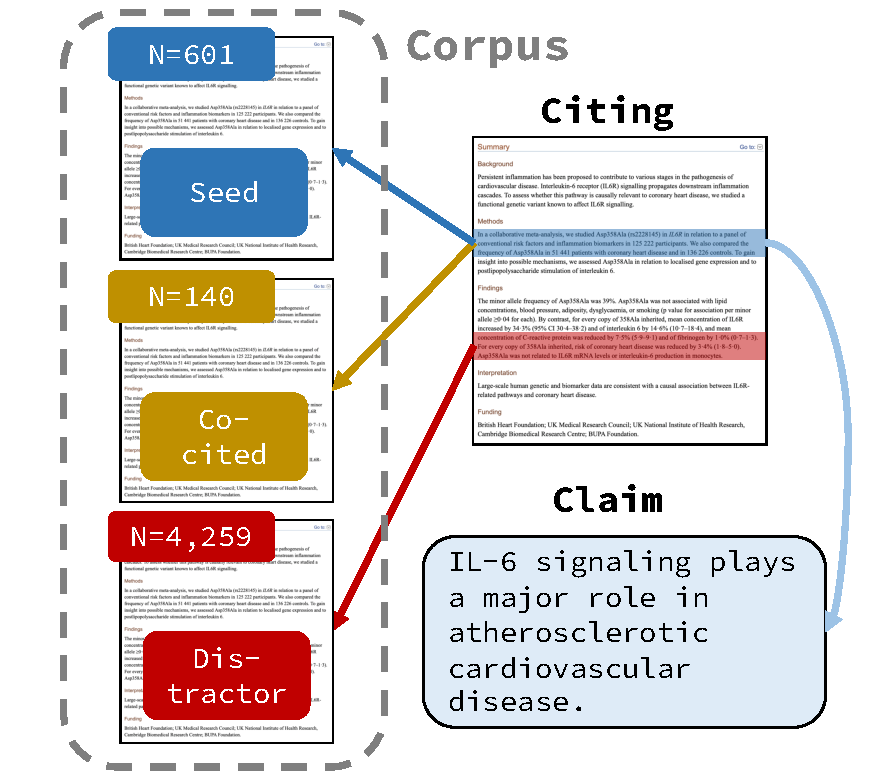
\includegraphics[width=\columnwidth, height=6.5cm]{figures/corpus-fig.pdf}
  \caption{Corpus construction. Citing abstracts are identified for each seed document. A claim is written based on the source citance in the citing abstract.}
  \label{fig:corpus}

\end{figure}

%%%%%%%%%%%%%%%%%%%%%%%%%

\subsection{Claim writing} \label{sec:claim_writing}
\noindent {\bf Annotation}
Annotators are shown a source citance in the context of an article, and are asked to write up to three claims based on the content of the citance. This results in \emph{natural} claims because the annotator does not see the cited article's abstract -- the \emph{cited abstract} -- at the time of claim writing. They are asked to skip citances that do not make statements about specific scientific findings. All annotators for both claim writing and verification were advanced undergraduate or graduate students with training in the life sciences.


\vspace{.2cm} \noindent{\bf Claim negation} Unless the authors of the source citance were mistaken, cited articles should provide supporting evidence for the claims made in a citance. To obtain examples where an abstract \refutes a claim, a scientific NLP expert wrote negations of existing claims, taking precautions not to bias the negations by relying on obvious keywords like ``not'' \cite{Schuster2019TowardsDF}.


%%%%%%%%%%%%%%%%%%%%

\subsection{Claim verification}
\label{sec:claim_verification}

\noindent {\bf Annotation} For each claim, all of the claim's cited abstracts are annotated for evidence. Annotators are shown a single claim / cited abstract pair, and asked to label the pair as \supports, \refutes, or \notenough. Although our task definition allows for a single claim to be both supported and refuted (by different abstracts) -- an occurrence we observe on real-world COVID-19 claims (\S\ref{sec:covid}) -- this never occurs in our dataset. Each claim has a single label. Counts for each label are shown in Table \ref{tbl:label_counts}. Overall, the annotators found evidence in 63\% of cited abstracts.  If the annotator assigns a \supports or \refutes label, they must also identify all rationales as defined in \S\ref{sec:evidence}. Table \ref{tbl:evidence_counts} provides statistics on the number of sentences per rationale, the number of rationales per claim / abstract pair, and the number of evidence abstracts per claim.  No abstract has more than 3 rationales for a given claim, and all rationales consist of at most three sentences. Rationales in \ours are mutually exclusive. 28 rationales contain non-contiguous sentences.

\ours claims are verified against abstracts rather than full articles since (1) abstracts can be annotated more scalably, (2) evidence is found in the abstract in more than 60\% of cases, and (3) previous attempts at full-document annotation suffered from low annotator agreement (\S\ref{sec:related_scinlp}).

\begin{table}[t]
  \setlength{\tabcolsep}{.25em}
  \footnotesize
  \centering


  \begin{subtable}{\linewidth}
    \begin{tabular}{L{0.12\linewidth} C{0.19\linewidth} C{0.19\linewidth} C{0.19\linewidth} C{0.15\linewidth}}
      \toprule
      Fold &  \supports &  \notenough &  \refutes &   All \\
      \midrule
      Train &       332 &              304 &      173 &   809 \\
      Dev   &       124 &              112 &       64 &   300 \\
      Test  &       100 &              100 &      100 &   300 \\
      \midrule
      All   &       556 &              516 &      337 &  1409 \\
      \bottomrule
    \end{tabular}
    \subcaption{Distribution of claim labels in \ours.}
    \label{tbl:label_counts}
  \end{subtable}

  \vspace{0.25em}

  \begin{subtable}{\linewidth}
    \begin{tabular}{L{0.48\linewidth} C{0.1\linewidth} C{0.1\linewidth} C{0.1\linewidth} C{0.1\linewidth}}
      \toprule
      {} &    0 &     1 &    2 &   3+ \\
      \midrule
      Cited abstracts per claim     &    - &  1278 &   86 &   45 \\
      Evidence abstracts per claim &  516 &   830 &   37 &   26 \\
      Rationales per abstract         &    - &   552 &  290 &  153 \\
      Sentences per rationale       &    - &  1542 &   92 &   11 \\
      \bottomrule
    \end{tabular}
    \subcaption{Evidence counts at various levels of granularity. For example, Column 2 of the row ``Rationales / abstract'' indicates that 290 claim / abstract pairs are supported by 2 distinct rationales.}
    \label{tbl:evidence_counts}
  \end{subtable}

  \caption{Statistics on claim labels, and the number of evidence abstracts and rationales per claim.}
  \label{tbl:evidence_stats}


\end{table}

\vspace{.2cm} \noindent{\bf Quality}
We assign \nagreement claim-abstract pairs for independent re-annotation. The label agreement is \labelkappa Cohen's $\kappa$, comparable with the 0.68 Fleiss' $\kappa$ reported in \citet{Thorne2018FEVERAL}, and 0.70 Cohen's $\kappa$ reported in \citet{Hanselowski2019ARA}. To measure rationale agreement, we treat each sentence as either classified as ``part of a rationale'' or ``not part of a rationale'' and compute sentence-level agreement on abstracts where annotators agreed on the \entailment label. The resulting Cohen's $\kappa$ is \rationalekappaagree.
